\documentclass[10pt]{article}
\usepackage[margin=1in]{geometry}
\usepackage{amsmath}
\usepackage{graphicx}
\usepackage{authblk}

\title{Benchmarking Data Assimilation Methods for Near-Wall Flow Reconstruction}
\author{Ángel González Villatoro}

\begin{document}
\maketitle

\begin{abstract}
Accurate reconstruction of near-wall flow structures is crucial for advancing experimental and numerical methods in fluid dynamics. This study evaluates several data assimilation (DA) strategies for reconstructing 2D unsteady wall-bounded flows from sparse synthetic sensor data, with a particular focus on temperature, pressure, and shear stress.

A sudden acceleration boundary layer model governed by the Navier-Stokes and energy equations is used as a testbed. High-resolution simulations serve as the reference dataset (800$\times$800), from which synthetic observations are extracted and assimilated into a coarser-resolution simulation (25$\times$25). Four DA methods are benchmarked: nudging, Kalman Filter (KF), Ensemble Kalman Filter (EnKF), and 4D-Var. Metrics include the root-mean-square error (RMSE), assimilation time, and a composite score balance (RMSE $\times$ time).

Results show that all methods achieve comparable accuracy (RMSE $\approx$ 0.1307), but differ in computational cost. Nudging and KF demonstrate the best trade-off between accuracy and efficiency, with nudging requiring less than 1 ms per update. EnKF allows multivariable assimilation with moderate overhead, while 4D-Var achieves high accuracy at the cost of significant computation.

This analysis highlights the potential of lightweight assimilation schemes for practical applications such as integrating surface-based techniques (e.g., TSP, PSP) into computational fluid dynamics workflows.


\begin{figure}[h]
\centering
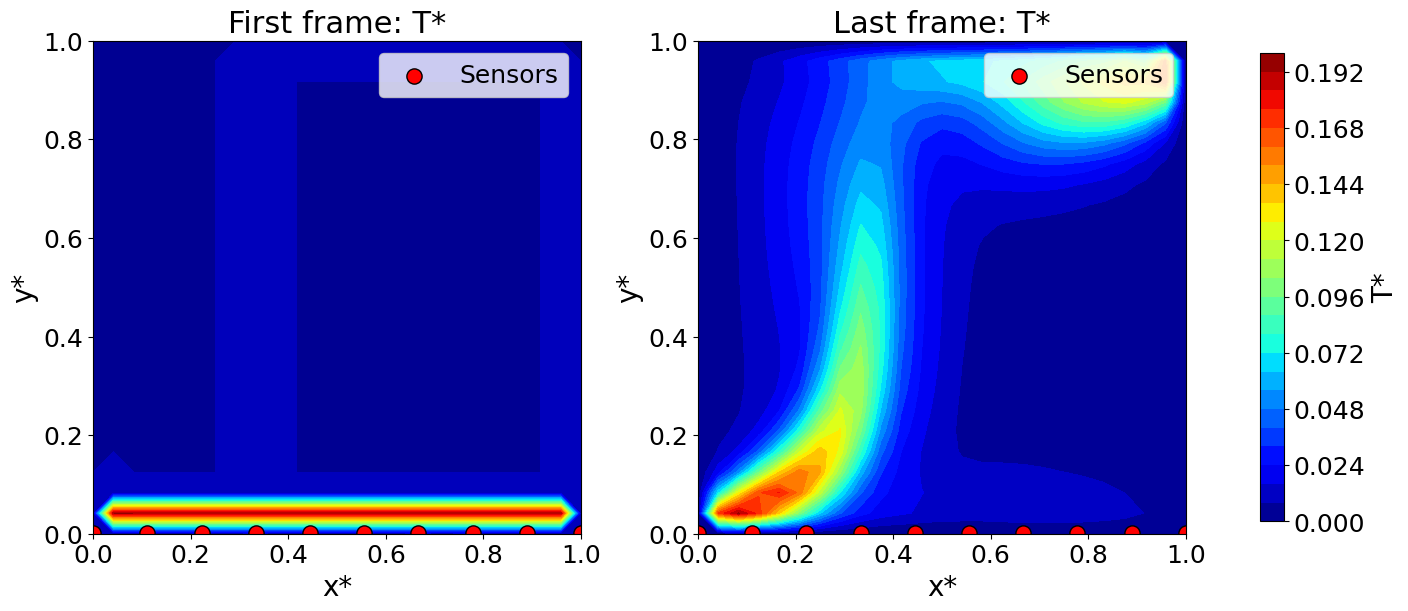
\includegraphics[width=0.8\textwidth]{output.png}
\caption{Simulation with implementation of data assimilation over temperature distribution for a flat plate suddenly accelerated.}
\end{figure}
\end{abstract}

\end{document}


